%!TEX root = ../masters_thesis.tex

\section{User Interface Design Process} % (fold)
\label{sec:user_interface_design_process}

The Hivent model presented in section \ref{sec:hivent_model} and the methods to edit the data in section \ref{sec:editing_hivent_data} serve as the foundation of HistoGlobe. However, the development of the system bottom-up from the data model to the interface might not lead to a usable system. Human-Centered Design promotes a top-down process from the user via the interface into the core of the application. This section illustrates the iterative design process for this thesis seen in figure \ref{fig:human_centered_design}

The two main use cases for HistoGlobe that are focused in this thesis are \emph{understanding} the history of countries and \emph{editing} it. The initial interviews confirmed that the combination of a map and a timeline are an appropriate way to interactively visualize the history of countries. Therefore, the main interface concept of HistoGlobe introduced in section \ref{sec:histoglobe} does not need to be changed. It is extended by the \emph{HistoGraph} introduced in section \ref{sub:histograph}. This promising set of visualizations forms the \emph{browsing mode} of HistoGlobe to understand the history of countries.

For editing purposes the idea of the \emph{edit mode}, a second interface mode, was developed. It is the main product of the iterative design process illustrated in this section. It is based on the edit operations, the workflow to edit the data and the concepts of retrospective updates and backward operations from section \ref{sec:editing_hivent_data}. The edit mode allows to intuitively edit Hivents, Areas and operations directly in HistoGlobe, without the need to write data into database tables.

% % - - - - - - - - - - - - - - - - - - - - - - - - - - - - - - - - - - - - - - -
% \paragraph{Initial interviews} % (fold)
% \label{par:initial_interviews}

% Four researchers were asked about their opinions on the idea of HistoGlobe, use cases and the concept of the edit mode. The idea proved popular, especially for students and teachers in school, historically interested people in general and also for scholars in digital humanities. All researchers agreed that the key to a successful interface is usability, because editing data in time and space is a challenging task. A main concern is uncertainty: Almost all sorts of information in historical research -- temporal, spatial and thematic -- are potentially uncertain. A good user interface for researchers therefore has to support uploading historical sources and indicating uncertainty.

% % paragraph initial_interviews (end)


% ------------------------------------------------------------------------------
\subsection{Paper Prototype} % (fold)
\label{sub:paper_prototype}

In the initial interviews it became clear that usability is the key to a successful interface that humanity scholars would actually use. In the second phase, the idea of the edit mode was developed as a paper prototype. It consists of a map of Europe, a timeline and a set of buttons and dialogs for the edit mode. The prototypes were evaluated with three test subjects. Each of them had to solve four tasks that cover different use cases and operations:
\begin{compactenum}
  \item 1300: Rename incorrectly spelled name of Switzerland on the map (\emph{correction})
  \item 1990: Unite East and West Germany (\emph{forward change})
  \item 1993: Separate the Soviet Union into Russia, Estonia, Latvia, etc. (\emph{forward change})
  \item 1944: Change the border between Finland and the Soviet Union before 1944 (\emph{backward change})
\end{compactenum}

\begin{figure}[ht]
  \centering
  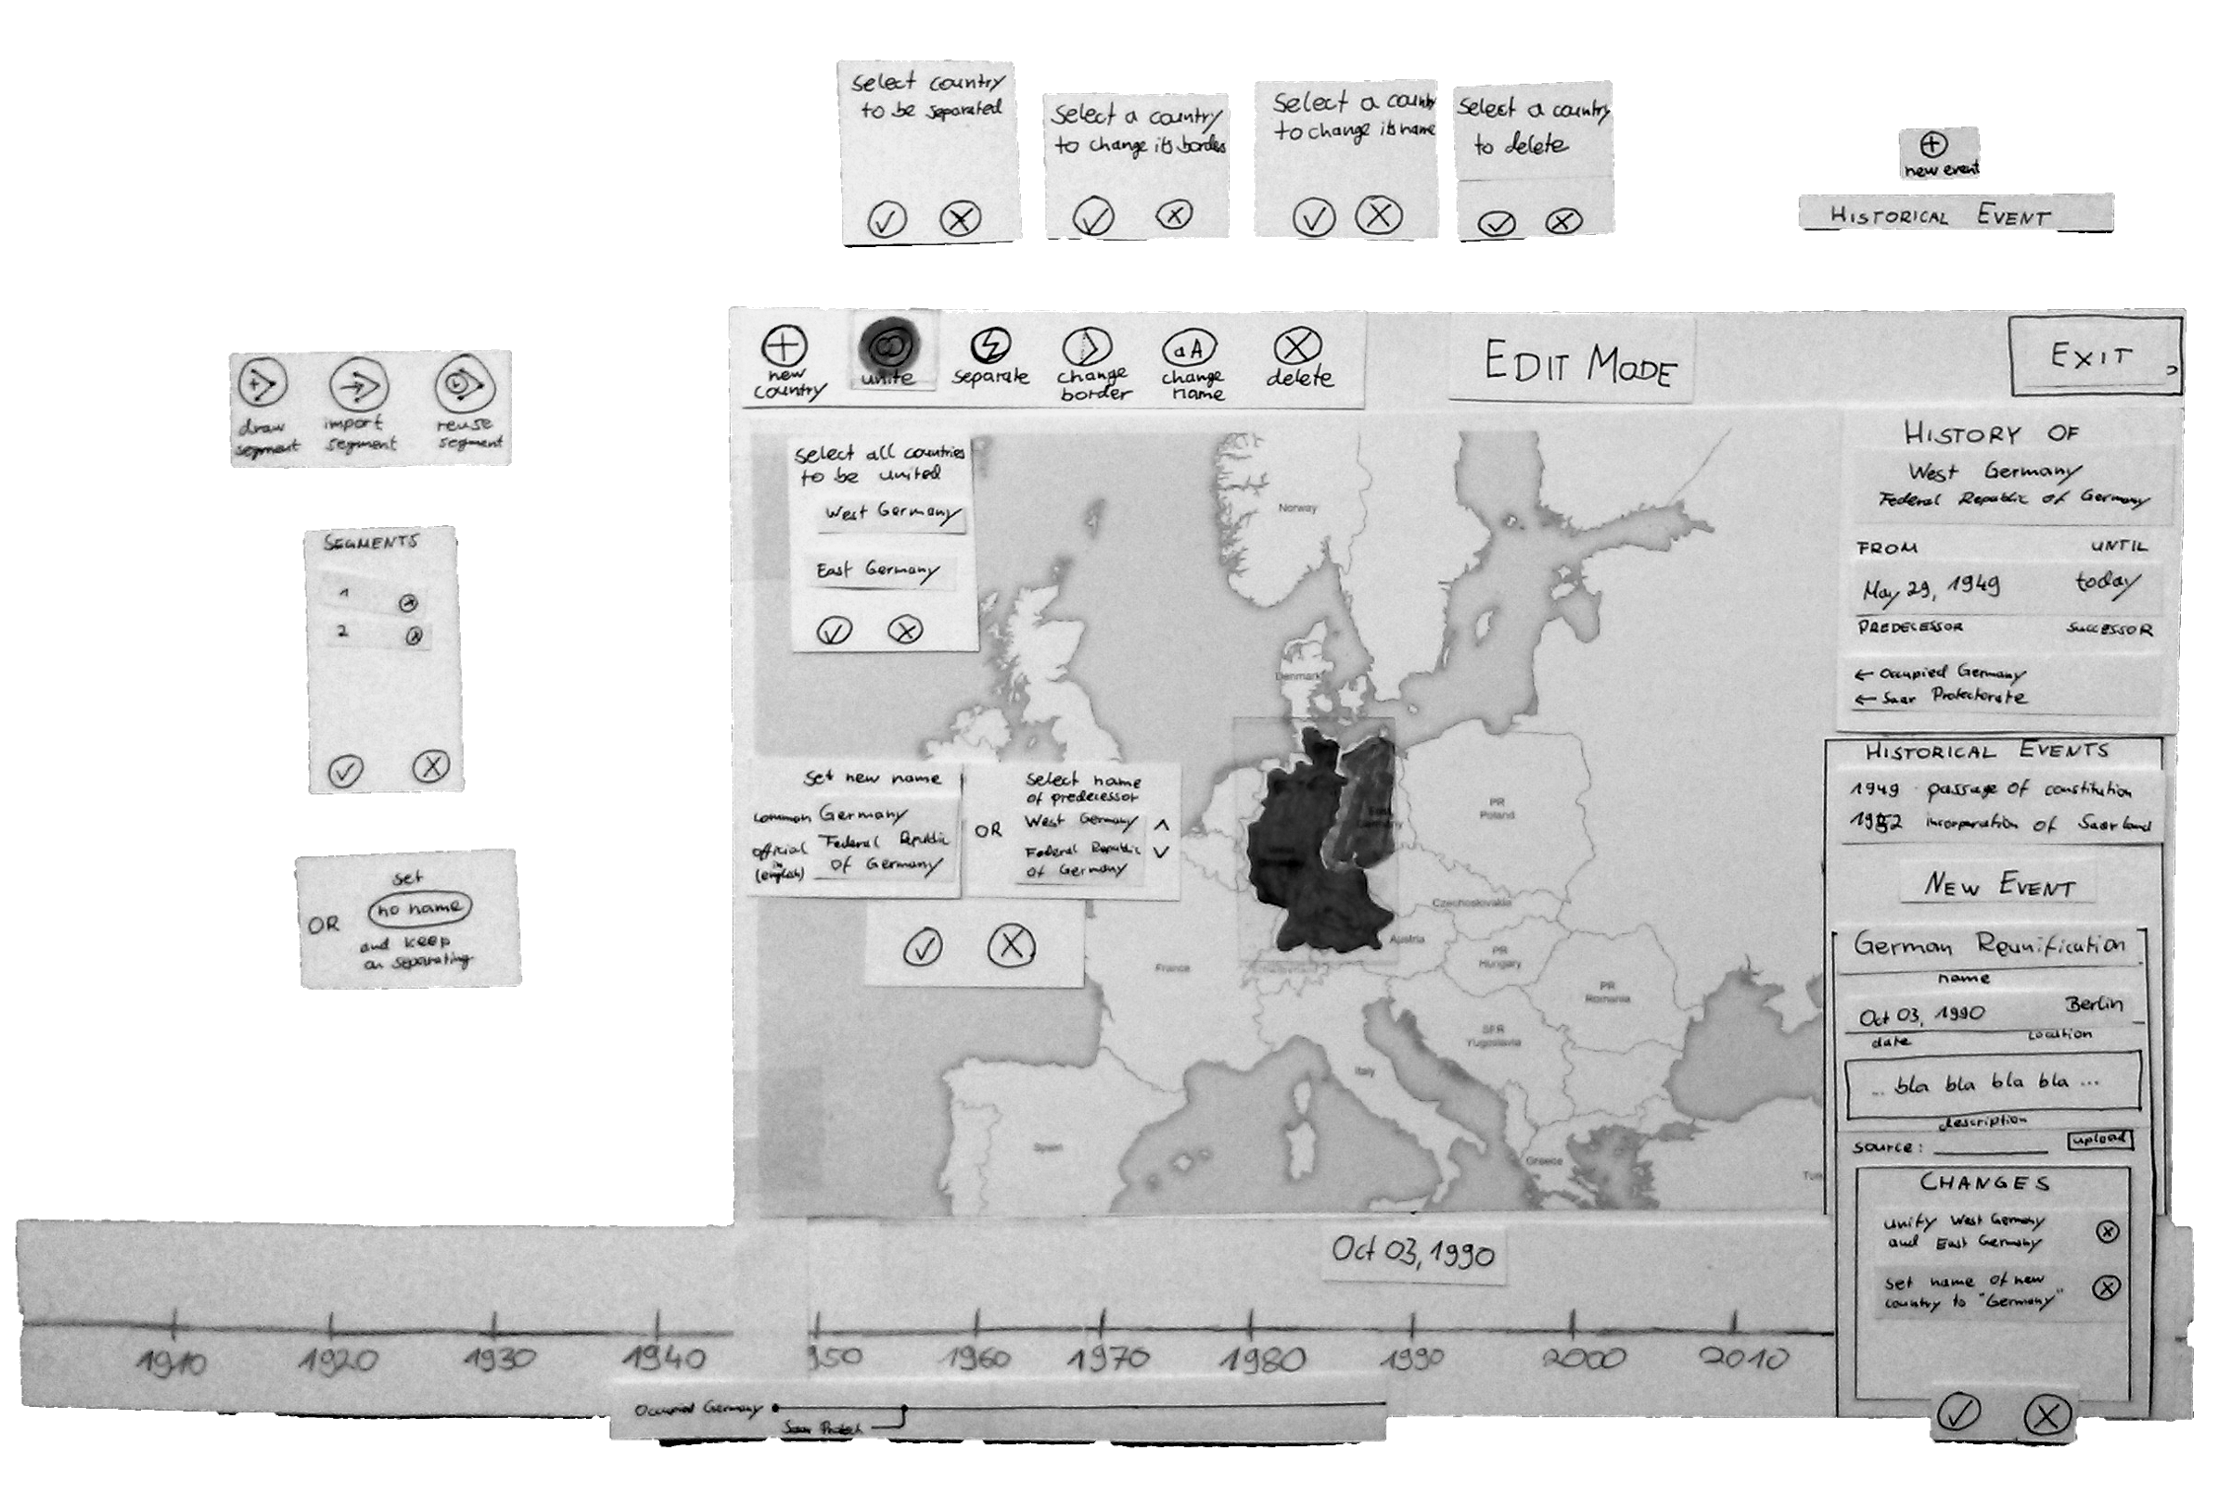
\includegraphics[width=0.9\textwidth]{graphics/development/user_interface_design_process/paper_prototype_2.png}
\caption{The second iteration of the paper prototype for the edit mode}
\label{fig:paper_prototypes}
\end{figure}

Two paper prototype iterations were created. Each iteration took about three full working days including the creation of the prototype, the conduction of the study and the analysis of the results. Finally, the concept was revised.
Most parts of the interface concept were understood and all subjects were able to solve the first three tasks. However, paper prototyping was very helpful to identify the following flaws early in the design process:

\begin{compactenum}
  \item The difference between Hivents, the history of a country and a historical change was unclear.
  \item The backward change was not understood.
  \item Correcting the name Switzerland by changing the event that created it in 1300 caused confusion.
\end{compactenum}

The main finding of this step was that depending on the task, there is both a Hivent-based and an Area-based mental model of the task. This became apparent in the edit operation for the German Reunification: some users started the unification operation first, and added West and East Germany afterwards -- and some selected first West Germany, then initiated a unification operation and then added East Germany. From that finding was concluded that the interface has to support both a Hivent-based and an Area-based approach to introduce historical changes and correct information on the map.

% subsection paper_prototype (end)

% - - - - - - - - - - - - - - - - - - - - - - - - - - - - - - - - - - - - - - -
\subsection{Mockup Prototype} % (fold)
\label{sub:mockup_prototype}

The main part of the design process was spent on the mockup prototypes. Their purpose is to rapidly develop an interface workflow that is understood by the users. The prototypes were created in \emph{LibreOffice Impress}, an open-source slide-based presentation tool. The interface is simulated on slides. The map is a background image, the timeline, the set of buttons and dialogs for the edit mode and HistoGraph are modeled with geometric elements, i.e.\ lines, circles and rectangles. Interactivity is simulated by linking a click on an element to a different slide that shows the effect of the operation. This allows the prototype to model sudden changes in the interface.

\begin{minipage}[t]{1.0\textwidth}

\vspace{1em}
\centering
\begin{figure}[H]
  \centering
  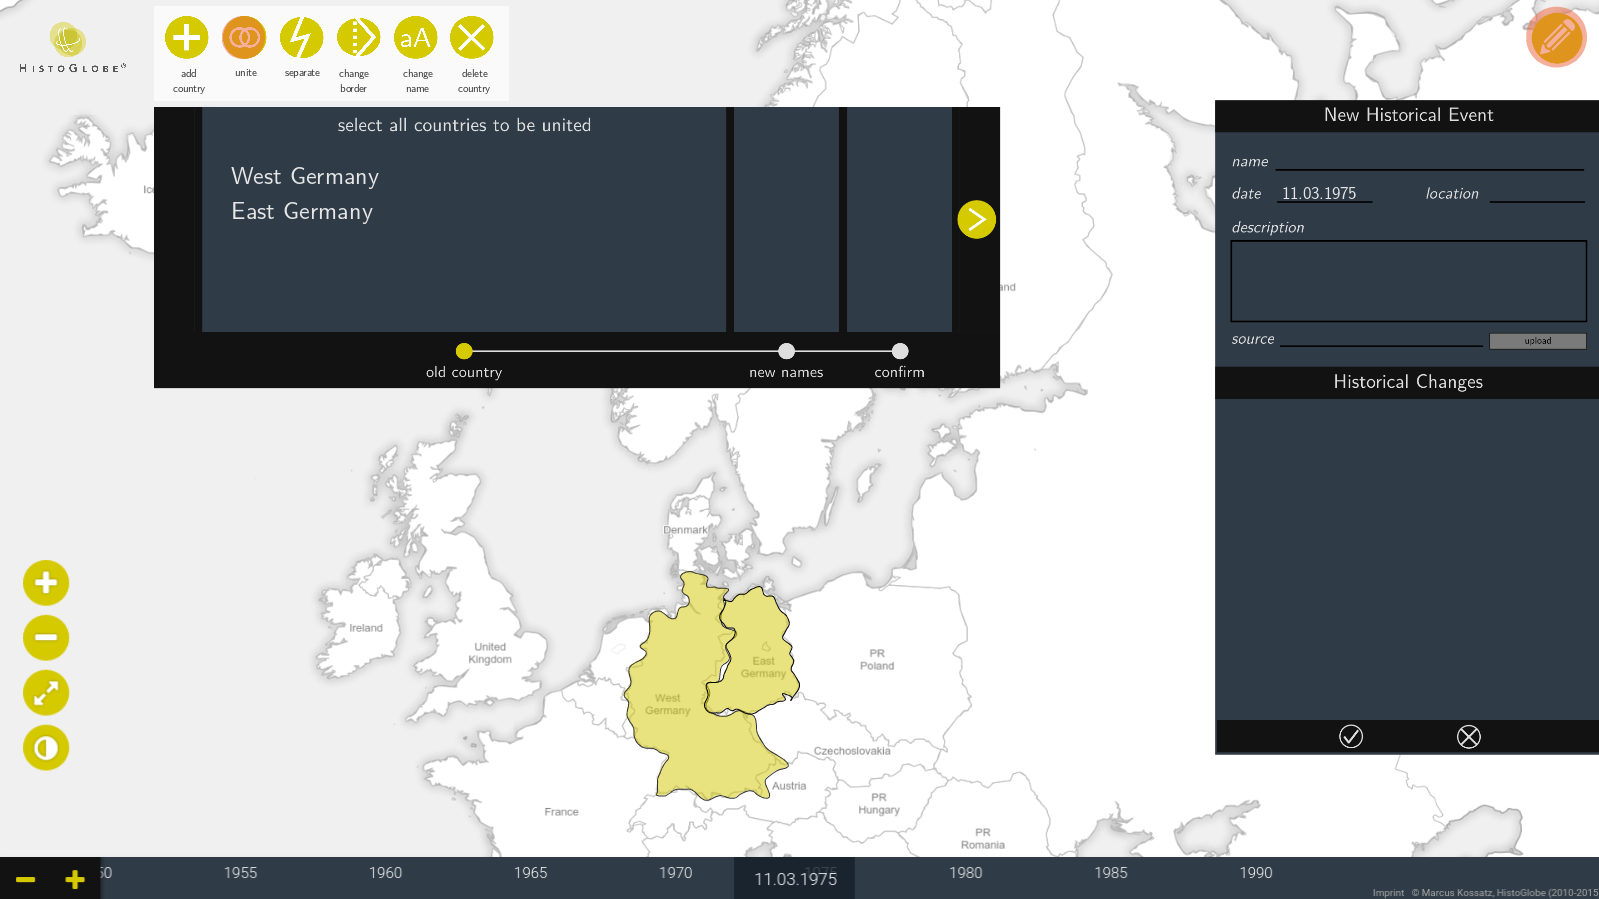
\includegraphics[width=0.75\textwidth]{graphics/development/user_interface_design_process/mockup_prototype_1.png}
\end{figure}
\begin{figure}[H]
  \centering
  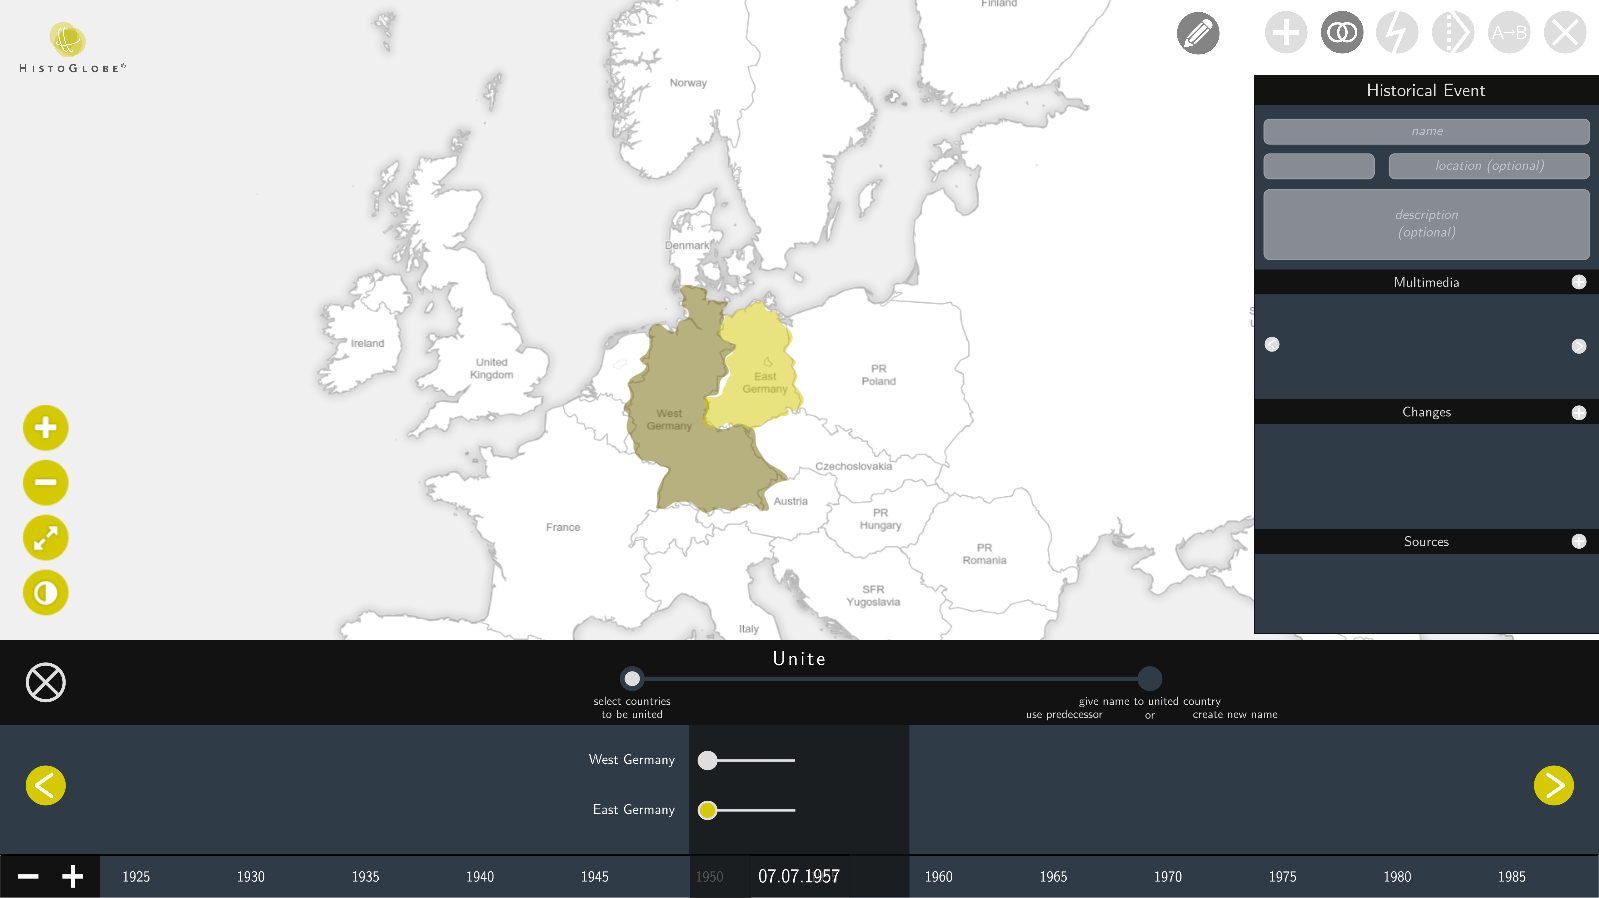
\includegraphics[width=0.75\textwidth]{graphics/development/user_interface_design_process/mockup_prototype_2.png}
\end{figure}
\begin{figure}[H]
  \centering
  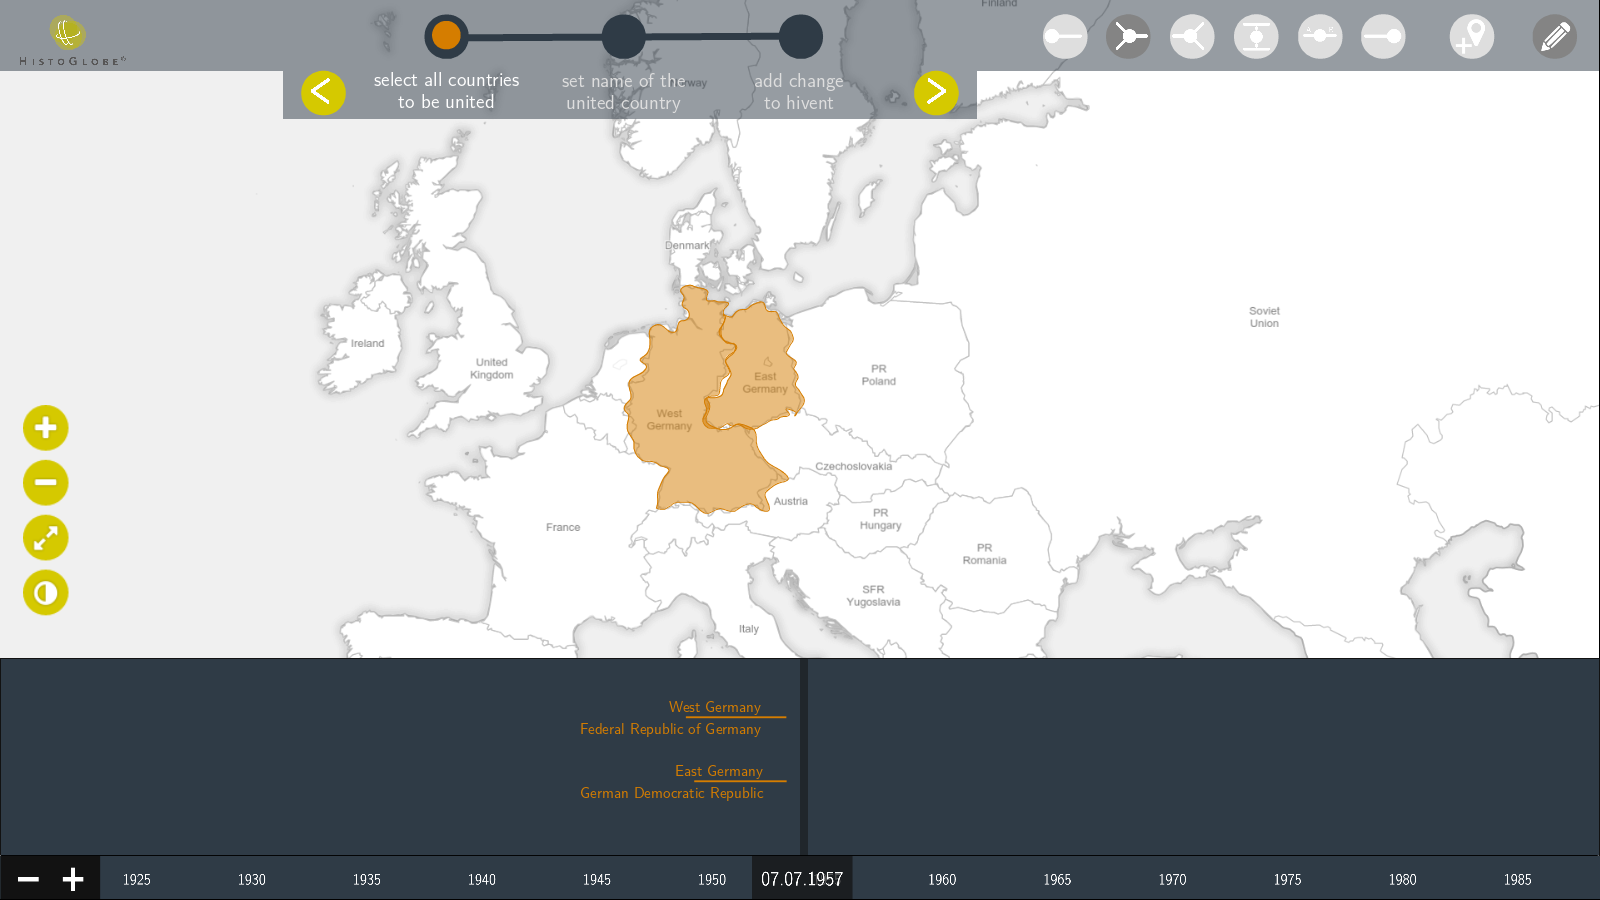
\includegraphics[width=0.75\textwidth]{graphics/development/user_interface_design_process/mockup_prototype_3.png}
  \caption{Three iteration stages of the mockup prototype for the edit mode}
  \label{fig:mockup_prototypes}
\end{figure}

\end{minipage}

Each prototype iteration was tested with multiple subjects and similar tasks as for the paper prototype. The interface was changed from one test to the next one. Several design problems, e.g.\ position of buttons, font sizes or color schemes were solved, but also conceptual issues arose.

\begin{quoteit}
  \begin{tabular}{l r}
    ``this was much easier than I thought'' ~~~~~~~~ &
    ``there is a training session needed'' \\[0.5em]
    ``the interface is very clear &
    ``the logic makes sense, \\
    and graphically pleasing'' &
    it is just very complex'' \\[0.5em]
    ``it's looking good'' &
    ``a nice tutorial and a good \\
    & documentation are necessary'' \\
  \end{tabular}
\end{quoteit}
\vspace{-1em}
\hfill -- quotes from the users of the mockup prototype

Especially the problem to initiate a retrospective update and a backward change proved to be very challenging. For each problem a design solution was developed. For retrospective updates, the interface needs to provide a visual clue where the next potential conflict arises. Figure \ref{sfig:retrospective_update} shows that West Germany can only be active until 1990, because then present-day Germany uses its territory. A button that flips an edit operation to initiate a backward operations is introduced in figure \ref{sfig:backward_change}: The \texttt{SEC} operation introduced to secede East Germany from Germany will be flipped into an \texttt{INC} operation to incorporate East Germany into Germany. The two gray Hivent markers on the left side of the timeline indicate that West and East Germany need a creation event, otherwise they would be active backwards all the way to $t_0$, the initial state of the system.

\begin{figure}[ht]
\centering
\begin{subfigure}[b]{.5\textwidth}
  \centering
  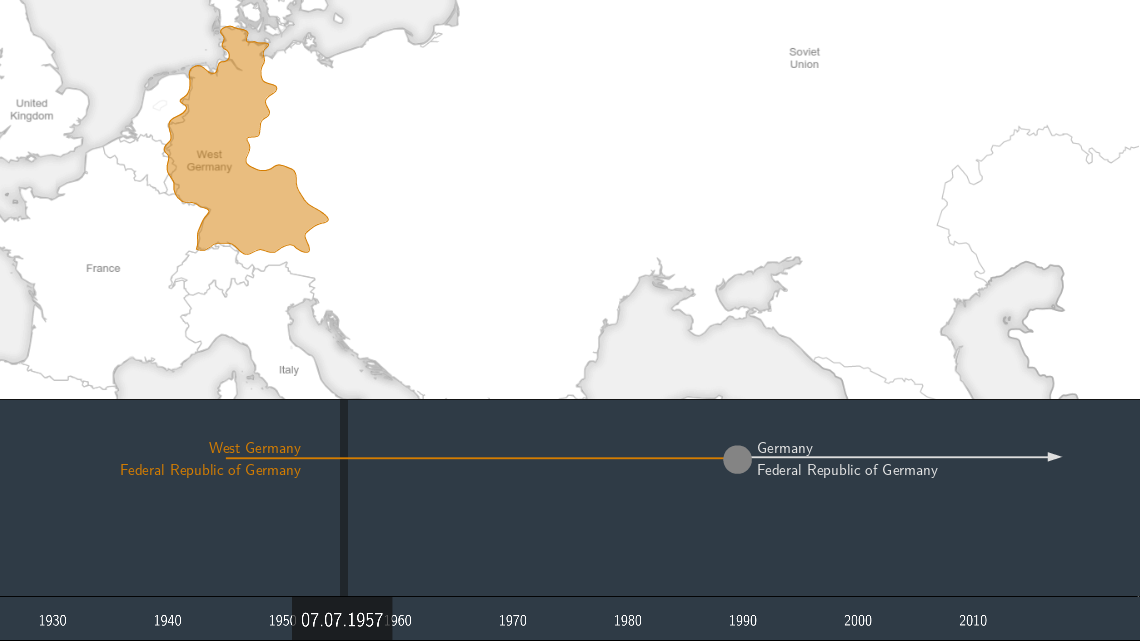
\includegraphics[width=200px]{graphics/development/user_interface_design_process/retrospective_update.png}
  \caption{Retrospective updates: visualizing the next conflict}
  \label{sfig:retrospective_update}
\end{subfigure}%
\begin{subfigure}[b]{.5\textwidth}
  \centering
  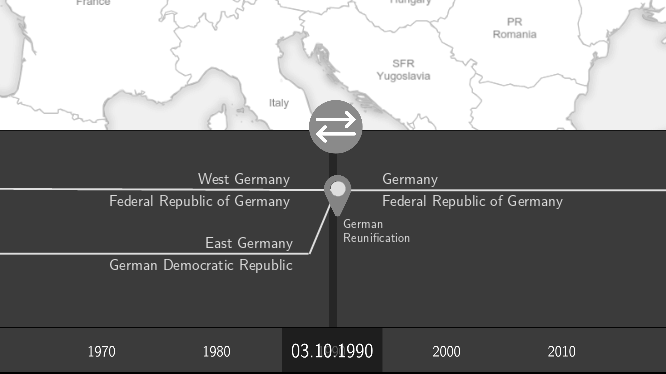
\includegraphics[width=200px]{graphics/development/user_interface_design_process/backward_change.png}
  \caption{Backward operation: flipping the edit operation}
  \label{sfig:backward_change}
\end{subfigure}
% \caption{Two approaches for editing changes backwards}
\label{fig:backward_change}
\end{figure}

The prototype was very valuable for the development process. In a total of two weeks, an interface concept and workflow was designed that the users understood. Its creation took longer than the paper prototype, but it was much faster than implementing an interactive web-based interface.


% subsection mockup_prototype (end)

% - - - - - - - - - - - - - - - - - - - - - - - - - - - - - - - - - - - - - - -
\subsection{Web-based prototype} % (fold)
\label{sub:web_based_prototype}

The main advantage of the design process so far is that it prevents major redesigns of the final web-based prototype. After three months of implementation time of the final system, the interface looks very similar to the last version of the mockup prototype. The main elements of the interface are the map, the timeline, the control buttons and the edit mode.

Not all desired features could be implemented:
As mentioned in section \ref{sub:histograph}, there were too many conceptual problems for the HistoGraph that had to be solved first.
Backward operations and retrospective updates are not supported as well, due to their complex nature in the computational model. The HistoGlobe version developed in this thesis only supports editing the history of countries with forward operations at the end of the timeline. The interaction and behavior is introduced in this section using the example of the fictional secession of Scotland from the United Kingdom in 2018.

\newpage
\begin{minipage}[t]{0.47\textwidth}

  \begin{figure}[H]
    \centering
    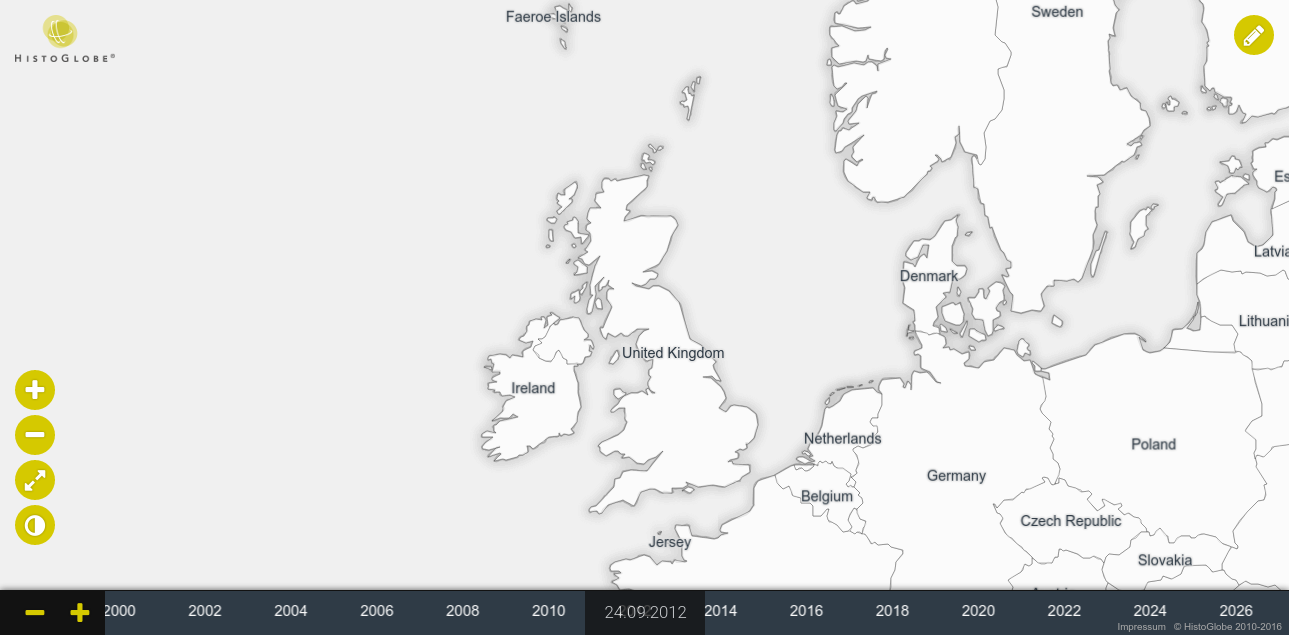
\includegraphics[width=1.0\textwidth]{graphics/development/user_interface_design_process/1_init.png}
    \caption{Initial state of the browsing mode}
    \label{fig:final_1_init}
  \end{figure}

  The initial state of the user interface. Additional to the original elements, there is an edit button on the upper right corner. A click on that button enters the edit mode of the system.

\end{minipage}    % N.B. the % is very important
\hspace{1.5em}    % N.B. this must go in this line, no blank lines !!!
\begin{minipage}[t]{0.47\textwidth}

  \begin{figure}[H]
    \centering
    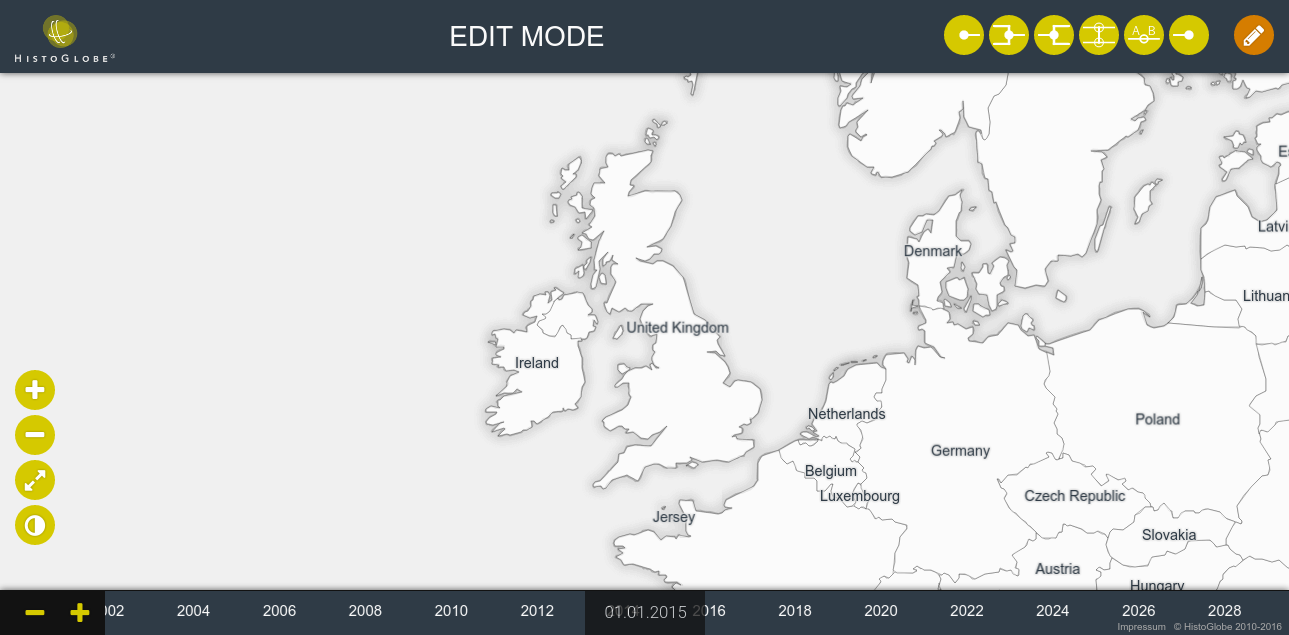
\includegraphics[width=1.0\textwidth]{graphics/development/user_interface_design_process/2_edit_mode.png}
    \caption{Initial state of the edit mode}
    \label{fig:final_2_edit_mode}
  \end{figure}

  In the edit mode, a title bar and six buttons for the edit operations appear. A click on one of these buttons starts the associated operation workflow as introduced in section \ref{sub:edit_workflow}.

\end{minipage}

\vspace{1em}
\begin{minipage}[t]{0.47\textwidth}

  \begin{figure}[H]
    \centering
    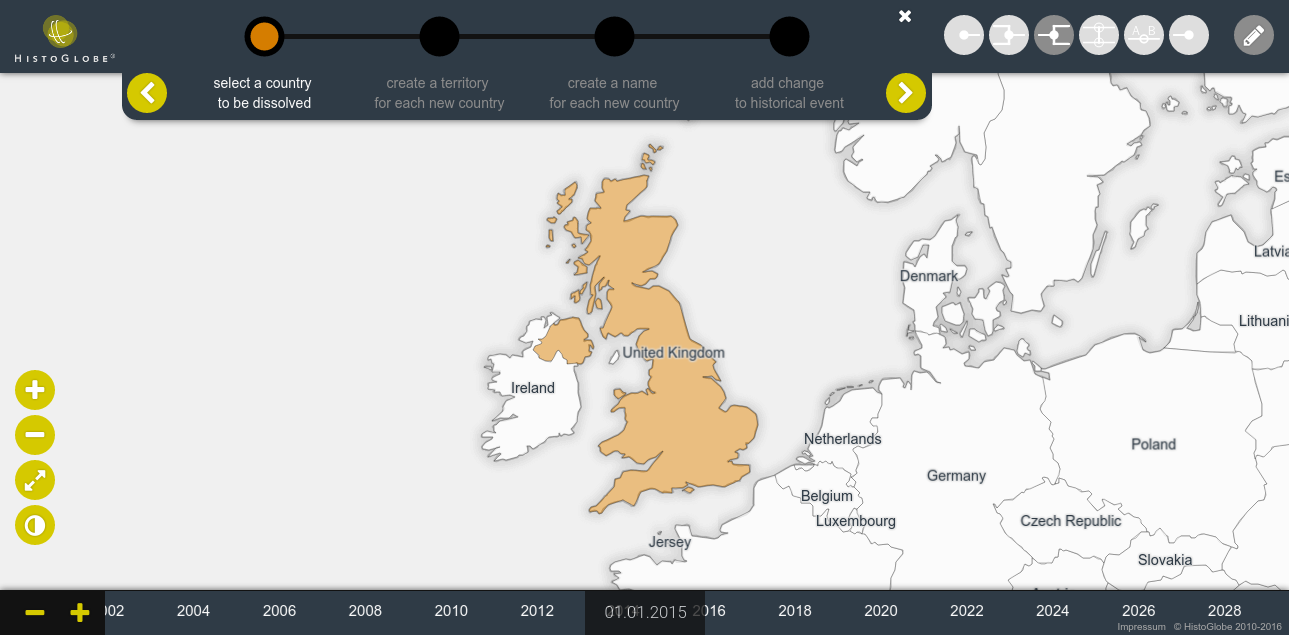
\includegraphics[width=1.0\textwidth]{graphics/development/user_interface_design_process/3_select_old_areas.png}
    \caption{1) Select old Areas}
    \label{fig:final_3_select_old_areas}
  \end{figure}

  A \emph{Workflow Window} guides the user step-by-step through the process of completing the edit operation. In case of \texttt{SPL}, the user has to select the country that he or she wants to be split via click on the map. After the step is completed, a click on the next button in the workflow window proceeds to the next step. At each point in the workflow, the back button reverts the previous action.

\end{minipage}    % N.B. the % is very important
\hspace{1.5em}    % N.B. this must go in this line, no blank lines !!!
\begin{minipage}[t]{0.47\textwidth}

  \begin{figure}[H]
    \centering
    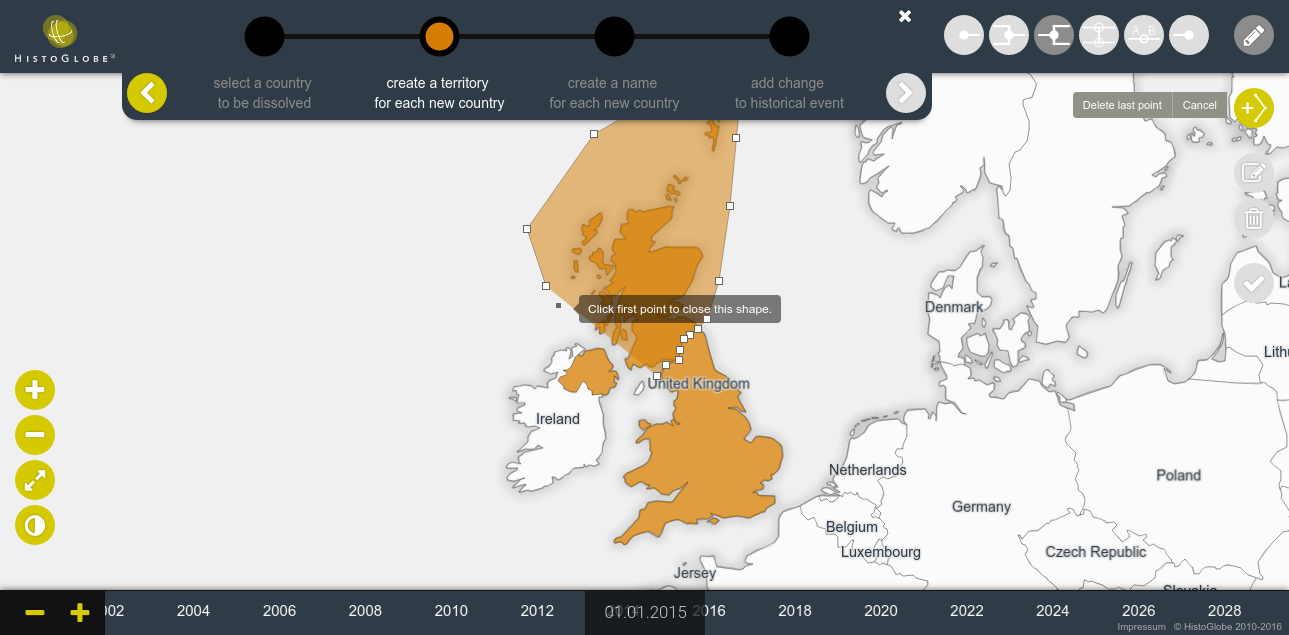
\includegraphics[width=1.0\textwidth]{graphics/development/user_interface_design_process/4_set_new_territories.png}
    \caption{2) Set a new territory}
    \label{fig:final_4_set_new_territories}
  \end{figure}

  In step two, the user has to create a territory for each new Area. The \emph{New Territory Tool} provides the option to create, manipulate and delete polygons directly on the map. The drawn polypolygon is intersected with the old territory to create the new Area. After at least one new territory has been created successfully, the remaining old territory can be selected on the map and finally be used as the last territory. If the entire old territory is distributed among the new Areas, the workflow proceeds to the next step.

\end{minipage}

\vspace{1em}
\begin{minipage}[t]{0.47\textwidth}

  \begin{figure}[H]
    \centering
    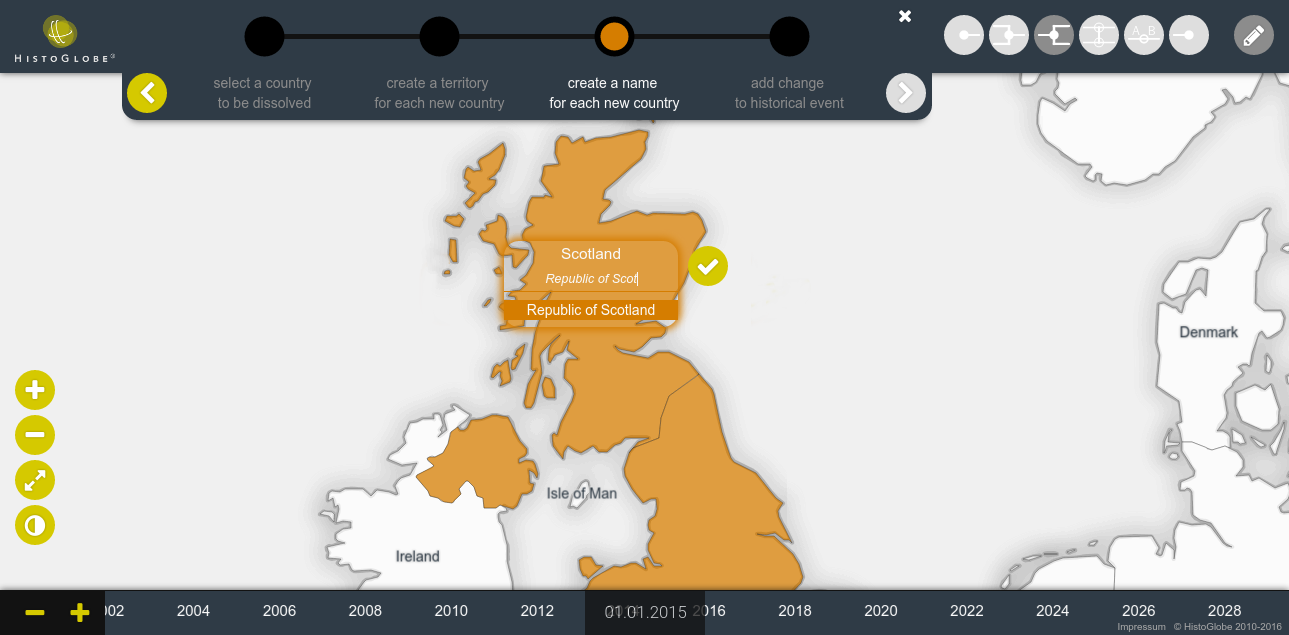
\includegraphics[width=1.0\textwidth]{graphics/development/user_interface_design_process/5_set_new_name.png}
    \caption{3) Set a new name}
    \label{fig:final_5_set_new_name}
  \end{figure}

  In the next step, the user has to define a name for each Area that has just been created. The \emph{New Name Tool} is a draggable box with two lines for the short and formal name. The user can make use of instant search to select existing country names from the database to be applied. The short name is put directly on the map once the confirm button is pressed.

\end{minipage}    % N.B. the % is very important
\hspace{1.5em}    % N.B. this must go in this line, no blank lines !!!
\begin{minipage}[t]{0.47\textwidth}

  \begin{figure}[H]
    \centering
    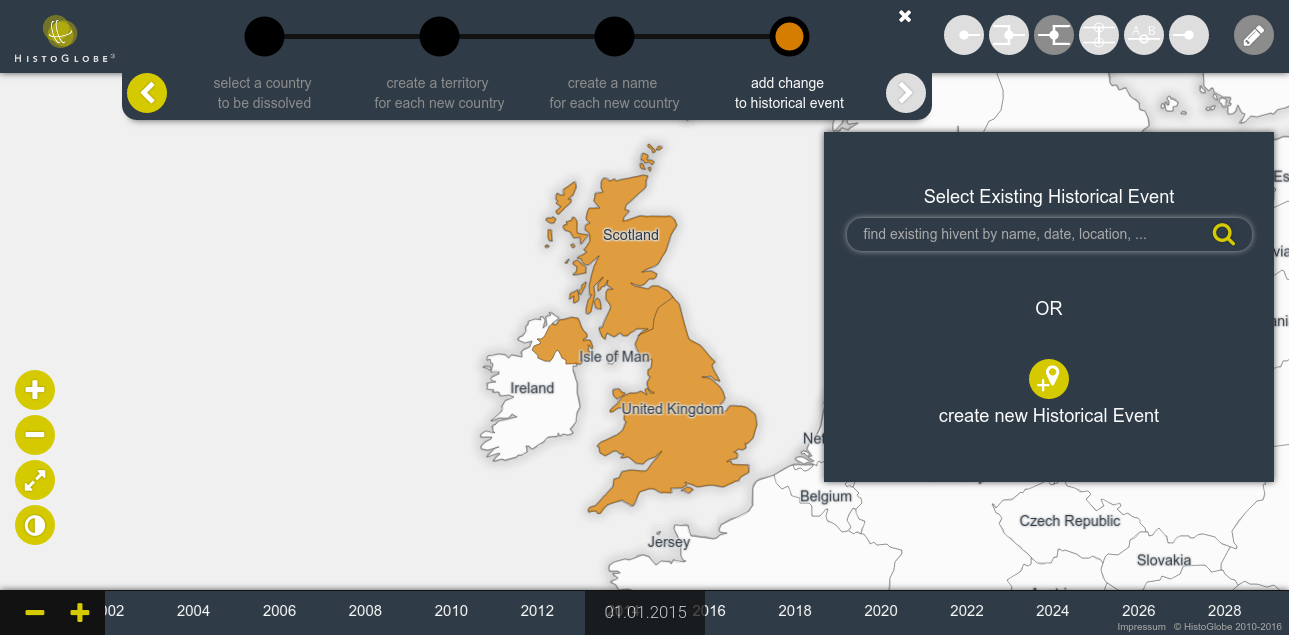
\includegraphics[width=1.0\textwidth]{graphics/development/user_interface_design_process/6_add_change_to_hivent_1.png}
    \caption{4) Add the Operation to a Hivent}
    \label{fig:final_6_add_change_to_hivent_1}
  \end{figure}

  When all names are set, the edit operation is complete. It has to be added to an Hivent in the last step of the workflow. The \emph{New Hivent Box} offers two options: either search for an existing Hivent add the edit operation to it or create a new Hivent.

\end{minipage}

\vspace{1em}
\begin{minipage}[t]{0.47\textwidth}

  \begin{figure}[H]
    \centering
    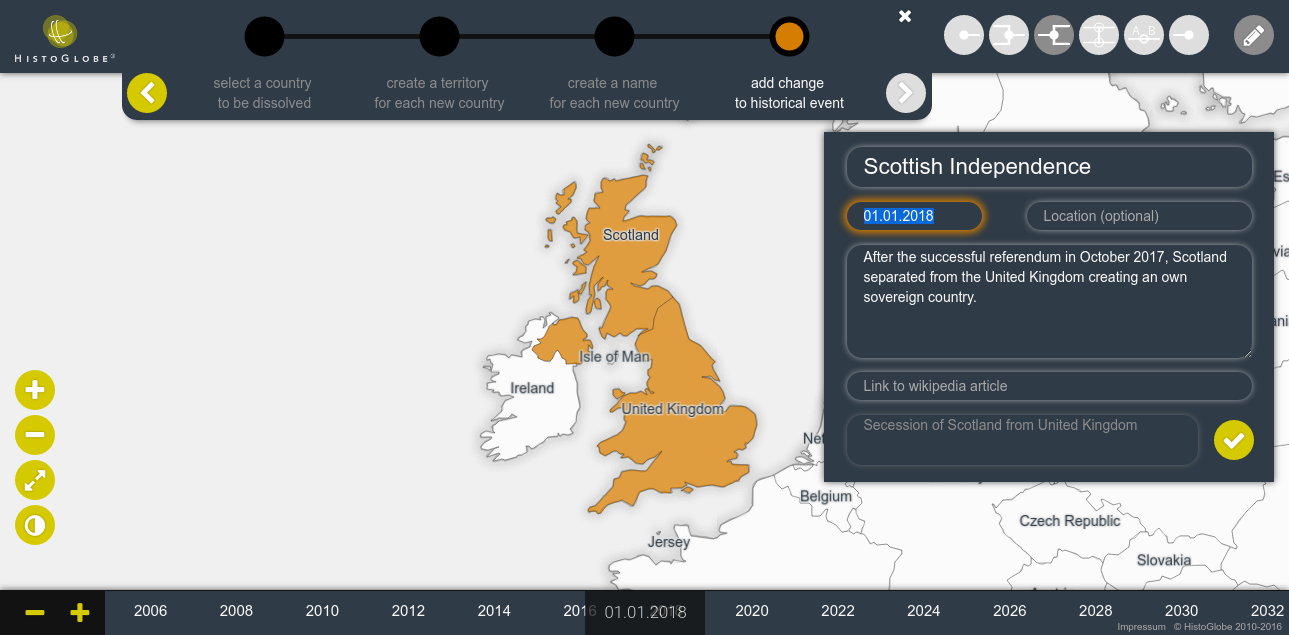
\includegraphics[width=1.0\textwidth]{graphics/development/user_interface_design_process/7_add_change_to_hivent_2.png}
    \caption{4) Create a new Hivent}
    \label{fig:final_7_add_change_to_hivent_2}
  \end{figure}

  The new Hivent created for that change is the ``Scottish Independence'' on 01.01.2018 with a description of the Hivent and optionally a location and a link to a Wikipedia article. In the last line, the historical change ``Secession of Scotland from the United Kingdom'' is noted. A click on the confirm button finalizes the edit operation workflow.

\end{minipage}    % N.B. the % is very important
\hspace{1.5em}    % N.B. this must go in this line, no blank lines !!!
\begin{minipage}[t]{0.47\textwidth}

  \begin{figure}[H]
    \centering
    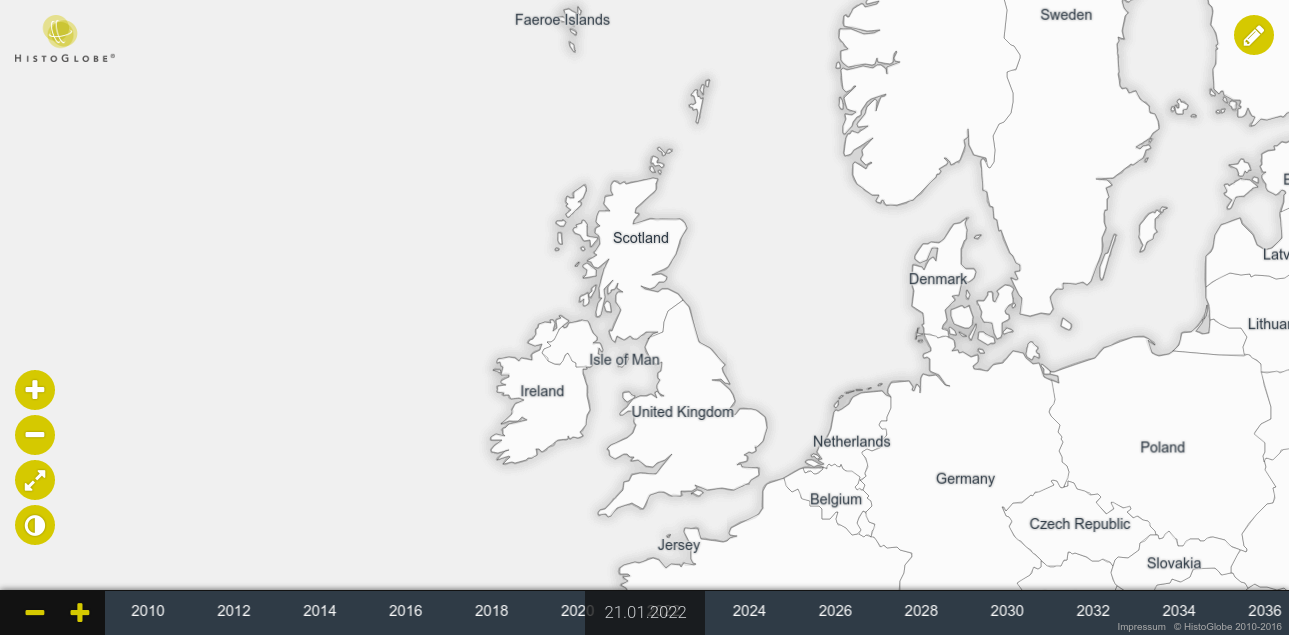
\includegraphics[width=1.0\textwidth]{graphics/development/user_interface_design_process/8_final_state.png}
    \caption{The final state with Scotland}
    \label{fig:final_8_final_state}
  \end{figure}

  A click on the edit button quits the Edit mode and returns to the browsing mode. Scotland and the United Kingdom are now separate Areas on the map after 2018. When the timeline is moved prior to 2018, Scotland is still part of the United Kingdom.

\end{minipage}

% subsection web_based_prototype (end)

% section user_interface_design_process (end)